

\section{Use Cases der Webanwendung} 

\subsection{Use Case-Diagramm}

Die Abbildung 5.2 veranschaulicht ein Use Case-Diagramm der Webanwendung.
Hier werden Interaktionsm\"oglichkeiten des Arztes mit der Software und die Kommunikation der 
Software mit dem Webserver dokumentiert.\\

\begin{figure}[h]
  \centering
  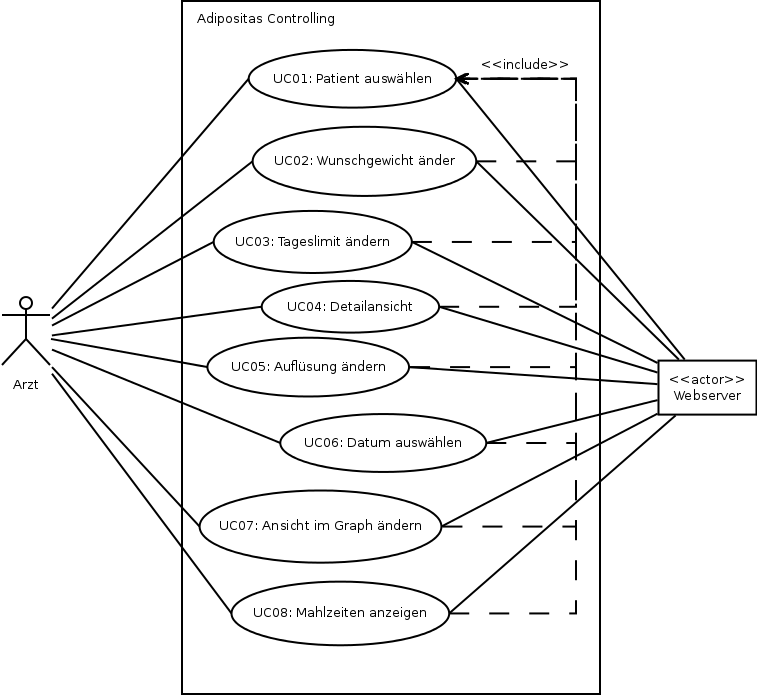
\includegraphics[scale=0.55]{diagramme/kapitel5/ac_usecases.png}
  \caption{Use Case-Diagramm der Controlling-Software}
  
\end{figure}

\subsection{Aktoren}

\begin{itemize}
 \item Arzt: Benutzer der Webanwendung
 \item Webserver: Webserver mit Service zum Auslesen der Tagesprotokolle aus der Datenbank.
\end{itemize}

\subsection{Use Case Kurzbeschreibungen}

\begin{itemize}
 \item UC01: Patient ausw\"ahlen\\
 Der Arzt w\"ahlt einen Patienten aus einer Liste aus.
 \item UC02: Wunschgewicht \"andern\\
 Der Arzt tr\"agt ein neues Wunschgewicht f\"ur den Patienten ein.
 \item UC03: Tageslimit \"andern\\
 Der Arzt tr\"agt eine Begrenzung an erlaubten Kilokalorien pro Tag f\"ur den Patienten ein.
 \item UC04: Detailansicht\\
 Der Arzt wechselt zur Detailansicht eines Patienten.
 \item UC05: Aufl\"osung \"andern\\
 Der Arzt \"andert die zeitliche Aufl\"osung der Graphen.
 \item UC07: Ansicht im Graphen \"andern\\
 Der Arzt \"andert die Ansicht von Informationen, welche im Graphen angezeigt werden.
 \item UC08: Mahlzeiten anzeigen\\
 Der Arzt wechselt zur Listenansicht von Mahlzeiten des Patienten.
\end{itemize}
